\section{Additional economic trajectories and receipt accounting}
\label{app:economic-detail}

\subsection{Portfolio-preserving construction targets}

Sol's G20 New York negotiation illustrates why a development budget must specify which existing assets it preserves. At d235, accepting the actual \$400 offer would leave \$97 after transfer interest. Tested spare mortgages, redemption and four orange houses leave \$41 while preserving brown hotels. Six houses are also reachable with \$91 left if Sol liquidates brown development. At d257, a diagnostic branch replacing Grok's actual rejection with acceptance of Sol's \$250 offer permits six orange houses with \$64 remaining while preserving the browns. Thus the six-house target is unavailable under one portfolio-preservation condition and reachable under another. The branch does not establish that accepting the earlier terms was preferable or predict Grok's agreement. It clarifies the assets and income sacrificed by each feasible budget.

\subsection{Construction, realized income and inherited portfolios}

\begin{figure}[t]
\centering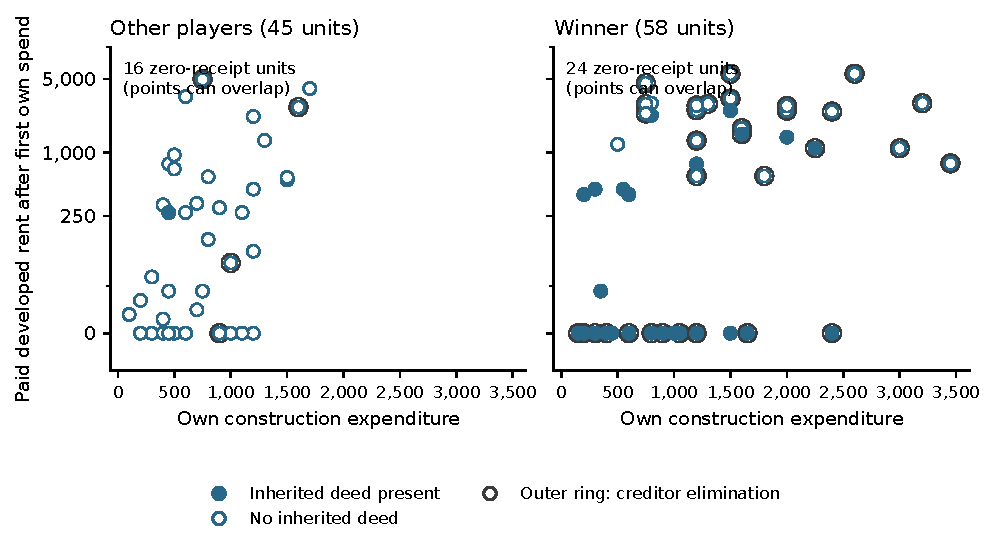
\includegraphics[width=\linewidth]{spending.pdf}
\caption{All 103 spending units, faceted by eventual winner status. Filled points contain an inherited deed at first own expenditure; outer rings indicate an elimination triggered by rent on that owner's group. The vertical axis is linear up to 250 and logarithmic above it. Forty units have zero paid developed receipts, with overlapping points on the baseline; twenty-six of them also trigger no creditor elimination. Receipts omit unpaid rent demands and are not net or incremental ROI. Winner status is a selected endpoint, not a treatment.}
\label{fig:spending}
\end{figure}

The 103 spending units incur \$103,450 in own construction expenditure. Whole-game paid developed rent to those units totals \$93,000, of which \$92,550 follows the owner's first own expenditure. The \$450 difference is G2 light-blue rent collected on inherited development before the winner's first own \$200 construction. Even the later window includes rent supported by inherited buildings. The totals describe expenditure and receipts on observed ownership paths; subtracting them does not yield net profit or construction's causal contribution.

Forty spending units collect no paid developed rent. Twenty-six of those also produce no creditor elimination on that group. These counts concern game/player/color units, whereas fifty-seven of sixty elimination events arise from rent on developed color properties. A large unpayable demand can end an opponent's game and transfer assets without appearing as a paid-rent receipt. Other zero-rent units retain assets, recover salvage, or face little remaining exposure. Denial and deterrence are possible sources of value but are not measured here. The data therefore support zero observed receipts, rather than forty failed investments.

Successive owners of G19's dark blues provide a concrete contrast. Opus spends \$1,200, receives \$175 in developed rent and later realizes \$600 in building sales. Gemini inherits the deeds, spends \$2,000 over its subsequent ownership, and receives \$1,400 in developed rent on a later Sol landing. The two units concern the same properties with different timing, financing and exposure. They show why an attractive group cannot guarantee receipts and why inherited ownership must remain visible. They do not isolate an owner effect. A recent \$1,200 construction step in the second trajectory must not be substituted for Gemini's \$2,000 cumulative own expenditure.

Winners account for fifty-eight spending units. Thirty-four contain at least one inherited deed at first own expenditure, while thirty first become complete through an estate. G3 brown, G6 light blue, G12 light blue and G14 green account for the distinction: inherited pieces are present, but later purchases or trades close the groups. A HOUSE\_BUILT-only definition would also miss G10's winner, which inherits four-house light blues and purchases \$150 in direct hotel conversions. The spending definition must include that case even though it records no own house purchase on the group.

Creditor inheritance is a major feature of the realized concentration of assets. The eventual winner is creditor in fifty-four of sixty eliminations, including thirty-five of forty nonterminal eliminations. Nineteen of twenty final eliminations name the winner as creditor; G13 ends with Luxury Tax owed to the bank. The nonterminal count is useful because it excludes estates received only when play has already ended. Under this implementation's declared variant, developed property can pass intact to a creditor. Productive assets accumulated by one player can consequently support another's later income and construction. The observed concentration is jointly determined by prior play, debts, movement and this rule. It is not a causal estimate of inheritance's advantage.
